The goal of this example was to achieve a muscle activation driven pointing task using a 2-DoF, 6-muscle arm model. 
In addition to muscle-induced torques, pure torques could compensate for the model weaknesses.
The movement lasted for 2 seconds and was discretized using 51 shooting nodes.

Term $\#1$ of the objective function (Tab.~\ref{tab:Muscle_activation_driven_pointing_task}) corresponds to the pointing tasks described by a Mayer term (heaviest weight), to superimpose two markers, the first one fixed in the ulna system of coordinates and the second one fixed in the scene.
Terms $\#2$ and $\#3$ were added for control regularization (muscle activation and torques) and $\#4$ for state regularization. 

%

%
\begin{table}[h!]
\caption{\small Objective terms of the activation-driven pointing task}
\label{tab:Muscle_activation_driven_pointing_task}
\centering
\begin{tabular}{c c c c}
\toprule 
& Type & Function & Weight \\ 
\midrule
$\#1$ & Mayer & ALIGN\_ MARKERS & $1e6$ \\ 
\midrule
$\#2$ & Lagrange & MINIMIZE\_ MUSCLE\_ CONTROL & $1e1$ \\ 
\midrule
$\#3$ & Lagrange & MINIMIZE\_ TORQUE & $1e1$ \\ 
\midrule
$\#4$ & Lagrange & MINIMIZE\_ STATE & $1e1$ \\
\bottomrule
\end{tabular}
\end{table}
%

%
The problem was solved with IPOPT and ACADOS resulting in two significantly different solutions with ACADOS proving a 16 times smaller optimized cost (Tab.~\ref{tab:Perfs_and_detailed_implementations_of_each_example}), which illustrate the pitfalls of local minima as well as the benefits of having access to different solvers with minimal effort.  
Indeed, the ACADOS-based solution (Fig.~\ref{fig:snapshots_activation_driven_pointing}, top) makes good use of gravity to minimize the control inputs, while the IPOPT-based solution (Fig.~\ref{fig:snapshots_activation_driven_pointing}, bottom) moved the arm in the opposite direction and was stuck in a local minimum (still achieving the task though). 
It is worth noting that no constraint was given about the shoulder range of motion to ensure physiological muscle trajectories. 
 
 

%
\begin{figure*}[t!]
\centering
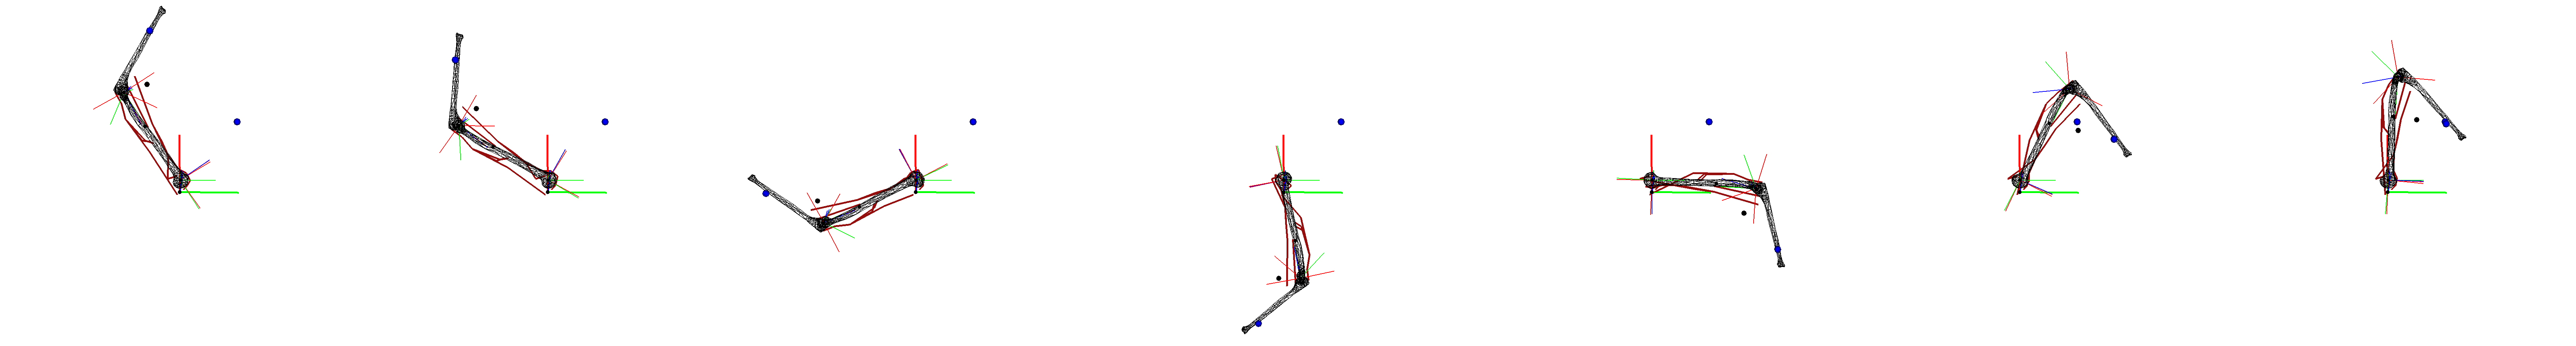
\includegraphics[width=\textwidth]{figures/activation_pointing_snapshots_acados.png}\\
\vspace*{0.5em}
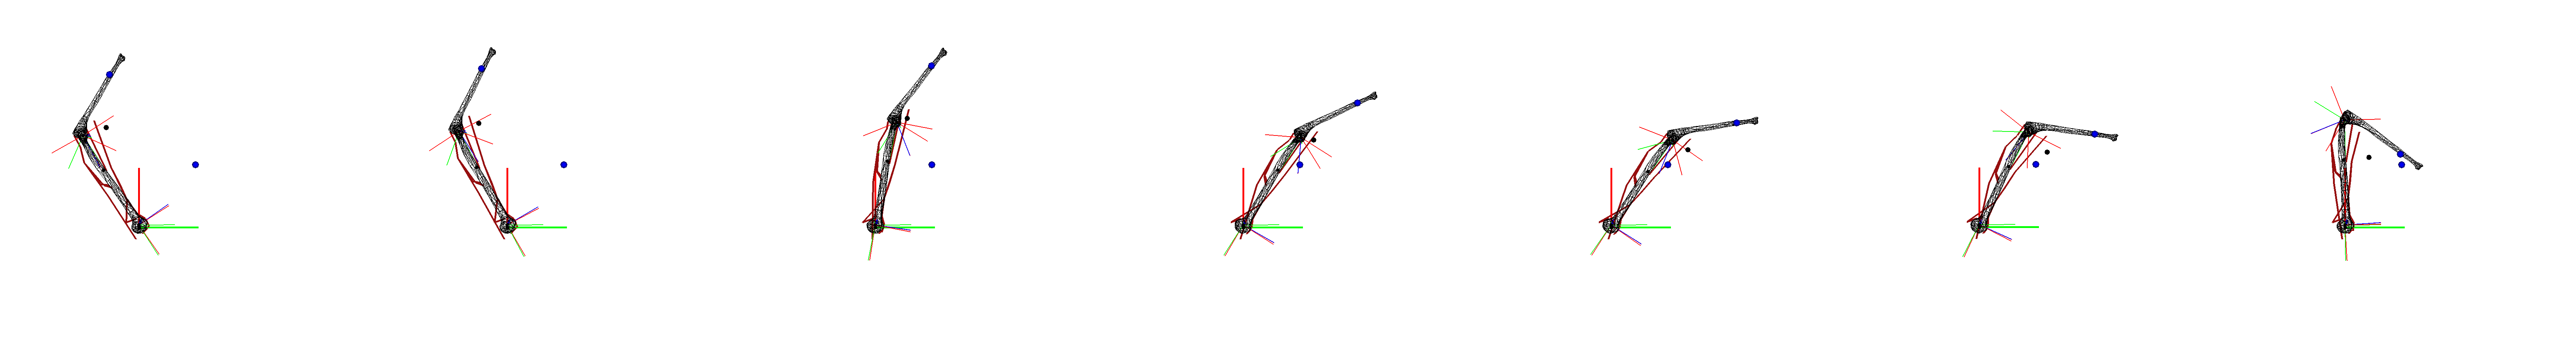
\includegraphics[width=\textwidth]{figures/activation_pointing_snapshots_ipopt.png}
\caption{Snapshots of an optimized muscle activation driven pointing task. Top: using ACADOS. Bottom: using IPOPT.}
\label{fig:snapshots_activation_driven_pointing}
\end{figure*}
%









